\section{Modelo Transformaciones y Herramientas}
\subsection{¿Qué es un modelo?}
El acrónimo MDD enfatiza el hecho de que los modelos son el foco central de MDD. Los modelos que nos interesan son aquellos relevantes para el desarrollo de software, sin embargo estos modelos no sólo representan al software; cuando un sistema de software soporta un determinado negocio, el modelo de dicho negocio es también relevante. Pero, ¿qué significa exactamente la palabra “modelo”? Necesitamos una definición que sea lo suficientemente general para abarcar varios tipos diferentes de modelos, pero que al mismo tiempo sea lo suficientemente específica para permitirnos definir transformaciones automáticas de un modelo a otro modelo. En el ámbito científico un modelo puede ser un objeto matemático (ej., un sistema de ecuaciones), un gráfico (ej., un plano) o un objeto físico (ej., una maqueta). El modelo es una representación conceptual o física a escala de un proceso o sistema, con el fin de analizar su naturaleza, desarrollar o comprobar hipótesis o supuestos y permitir una mejor comprensión del fenómeno real al cual el modelo representa y permitir así perfeccionar los diseños, antes de iniciar la construcción de las obras u objetos reales. Se utilizan con frecuencia para el estudio de represas, puentes, puertos, aeronaves, etc. Muchas veces, para obras complejas como por ejemplo una vivienda, se requiere la construcción de más de un modelo (figura 2-1). Por ejemplo, un modelo general de la disposición de los ambientes de la vivienda con sus puertas y ventanas, un modelo específico a una escala mayor para la instalación eléctrica y sanitaria, uno diferente para mostrar la estética de la fachada y el entorno, etc.
\\\\
\begin{figure}[H]
\centering
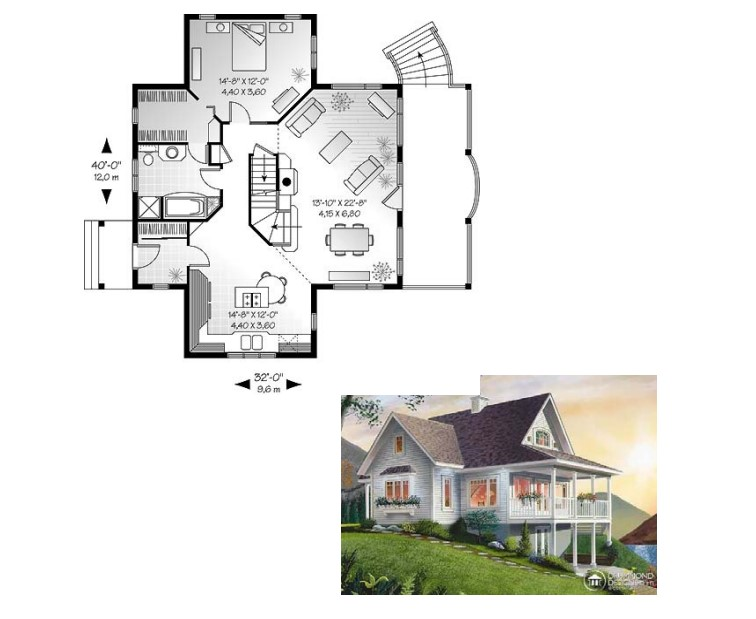
\includegraphics[scale=0.5]{./Imagenes/modelo1}
\caption{Ejemplo de figura 1-2}
\label{figura1}
\end{figure}

\subsection{Tipos de Modelos}
La definición de modelo dada en la sección anterior es muy amplia pues abarca muchos tipos diferentes de modelos. Los sistemas de software involucran varios modelos interdependientes a diferentes niveles de abstracción (análisis, diseño, implementación), representando diferentes partes del sistema (interfaz con el usuario, base de datos, lógica del negocio, administración del sistema), diferentes requisitos (seguridad, desempeño, flexibilidad), o diferentes tareas (modelos de pruebas, modelos de emplazamiento). En muchos casos, es posible generar un modelo a partir de otro, por ejemplo pasando del modelo de análisis al modelo de diseño, o del modelo de la aplicación al modelo de pruebas. Existen varias formas de distinguir entre tipos de modelos, cada una de ellas se basa en la respuesta a alguna pregunta acerca del modelo, por ejemplo:\\ \\
- ¿En qué parte del proceso de desarrollo de software es usado el modelo?\\
 - ¿El modelo es abstracto o es detallado?\\
 - ¿Qué sistema es descrito por el modelo? ¿Es un modelo del negocio o es un modelo de software?\\
 - ¿Qué aspectos del sistema son descritos por el modelo? ¿Es un modelo de la estructura o es un modelo del comportamiento?\\ 
- ¿Es un modelo orientado a una tecnología específica o es un modelo independiente de la tecnología?\\ \\
Las respuestas a estas preguntas nos permiten clasificar los diferentes tipos de modelos en categorías no disjuntas. En las siguientes secciones analizaremos en detalle esta clasificación.
\\\\

\subsection{Modelos a lo largo del proceso de desarrollo:}
Durante el proceso de desarrollo de software se crean diferentes modelos (figura 2-2). Los modelos de análisis capturan sólo los requisitos esenciales del sistema de software, describiendo lo que el sistema hará independientemente de cómo se implemente. Por otro lado, los modelos de diseño reflejan decisiones sobre el paradigma de desarrollo (orientado a objetos, basado en componentes, orientado a aspectos, etc.), la arquitectura del sistema (distintos estilos arquitecturales), la distribución de responsabilidades (GRASP patterns [Larman 04], GoF patterns [GHJV94]), etc. Finalmente, los modelos de implementación describen cómo el sistema será construido en el contexto de un ambiente de implementación determinado (plataforma, sistema operativo, bases de datos, lenguajes de programación, etc.). Si bien algunos modelos pueden clasificarse claramente como un modelo de análisis, o de diseño o de implementación, por ejemplo, un diagrama de casos de uso es un modelo de análisis, mientras que un diagrama de interacción entre objetos es un modelo de diseño y un diagrama de deployment es un modelo de implementación. En general, esta clasificación no depende del modelo en sí mismo sino de la interpretación que se de en un cierto proyecto a las etapas de análisis, diseño e implementación.
\begin{figure}[H]
\centering
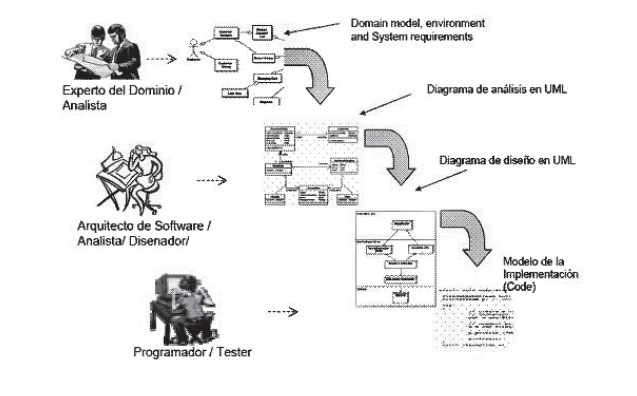
\includegraphics[scale=0.9]{./Imagenes/modelo2}
\caption{Ejemplo de figura 2}
\label{figura2}
\end{figure}

\subsection{Modelos abstractos y modelos detallados:}
 La clasificación entre modelo abstracto y modelo detallado también posee cierto grado de subjetividad. En general las herramientas de modelado nos permiten visualizar a un mismo modelo en distintos niveles de detalle [Egyed 02]. Por ejemplo podemos visualizar un diagrama de clases en forma abstracta limitando la información que se despliega sobre cada DESARROLLO DE SOFTWARE DIRIGIDO POR MODELOS clase sólo a su nombre, y limitando la profundidad de las jerarquías de herencia y composición a un máximo de k niveles. Luego podemos visualizar el diagrama en más detalle, incluyendo los nombres de los métodos públicos de cada clase y/o expandiendo las jerarquías de clases.
 
\subsection{Modelos de negocio y modelos de software:}
 Un modelo del negocio describe a un negocio o empresa (o parte de ellos). El lenguaje que se utiliza para construir el modelo del negocio contiene un vocabulario que permite al modelador especificar los procesos del negocio, los clientes, los departamentos, las dependencias entre procesos, etc. Un modelo del negocio no describe necesariamente detalles acerca del sistema de software que se usa en la empresa; por lo tanto a este modelo suele llamárselo “modelo independiente de la computación” (CIM). Cuando una parte del negocio es soportada por un sistema de software, se construye un modelo diferente para tal sistema. Este modelo de software es una descripción del sistema de software. El sistema de software y el sistema del negocio son conceptos diferentes en el mundo real, sin embargo los requisitos del sistema de software usualmente se derivan del modelo del negocio al cual el software brinda soporte. Para la mayoría de los negocios existen varios sistemas de software dándole soporte. Cada sistema de software se usa para asistir una parte del negocio. Por lo tanto, existe una relación entre un modelo del negocio y los diferentes modelos de software que describen al software que brinda soporte al negocio, como mostramos en la figura 2-3.
\begin{figure}[H]
\centering
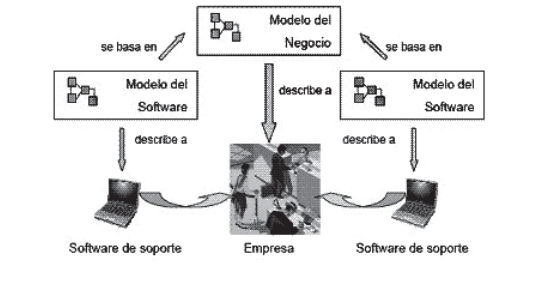
\includegraphics[scale=0.9]{./Imagenes/modelo3}
\caption{Ejemplo de figura 3}
\label{figura3}
\end{figure}

\subsection{Cualidades de los modelos:}
 El modelo de un problema es esencial para describir y entender el problema, independientemente de cualquier posible sistema informático que se use para su automatización. El modelo constituye la base fundamental de información sobre la que interactúan los expertos en el dominio del problema y los desarrolladores de software. Por lo tanto es de fundamental importancia que exprese la esencia del problema en forma clara y precisa. Por otra parte, la actividad de construcción del modelo es una parte crítica en el proceso de desarrollo. Los modelos son el resultado de una actividad compleja y creativa y por lo tanto son propensos a contener errores, omisiones e inconsistencias. La validación y verificación del modelo es muy importante, ya que la calidad del producto final dependerá fuertemente de la calidad de los modelos que se usaron para su desarrollo. Demos una mirada más detallada a las cualidades que esperamos encontrar en los modelos.\\\\ 
- Comprensibilidad. El modelo debe ser expresado en un lenguaje que resulte accesible (es decir entendible y manejable) para todos sus usuarios. \\\\
- Precisión. El modelo debe ser una fiel representación del objeto o sistema modelado. Para que esto sea posible, el lenguaje de modelado debe poseer una semántica precisa que permita la interpretación unívoca de los modelos. La falta de precisión semántica es un problema que no solamente atañe al lenguaje natural, sino que también abarca a algunos lenguajes gráficos de modelado que se utilizan actualmente.\\\\
- Consistencia. El modelo no debe contener información contradictoria. Dado que un sistema es representado a través de diferentes sub-modelos relacionados debería ser posible especificar precisamente cuál es la relación existente entre ellos, de manera que sea posible garantizar la consistencia del modelo como un todo. \\\\
- Completitud. El modelo debe capturar todos los requisitos necesarios. Dado que en general, no es posible lograr un modelo completo desde el inicio del proceso, es importante poder incrementar el modelo. Es decir, comenzar con un modelo incompleto y expandirlo a medida que se obtiene más información acerca del dominio del problema y/o de su solución.\\\\ 
- Flexibilidad. Debido a la naturaleza cambiante de los sistemas actuales, es necesario contar con modelos flexibles, es decir que puedan ser fácilmente adaptados para reflejar las modificaciones en el dominio del problema.\\\\
- Re-usabilidad. El modelo de un sistema, además de describir el problema, también debe proveer las bases para el re-uso de conceptos y construcciones que se presentan en forma recurrente en una amplia gama de problemas. \\\\
- Corrección. El análisis de la corrección del sistema de software debe realizarse en dos puntos. En primer lugar el modelo en sí debe ser analizado para asegurar que cumple con las expectativas del usuario. Este tipo de análisis generalmente se denomina ‘validación del modelo’. Luego, asumiendo que el modelo es correcto, puede usarse como referencia para analizar la corrección de la implementación del sistema Esto se conoce como ‘verificación del software’. Ambos tipos de análisis son necesarios para garantizar la corrección de un sistema de software.

\subsection{¿Qué es una transformación?}
 El proceso MDD, descrito anteriormente, muestra el rol de varios modelos, PIM, PSM y código dentro del framework MDD. Una herramienta que soporte MDD, toma un PIM como entrada y lo transforma en un PSM. La misma herramienta u otra, tomará el PSM y lo transformará a código. Estas transformaciones son esenciales en el proceso de desarrollo de MDD. En la figura 2-4 se muestra la herramienta de transformación como una caja negra, que toma un modelo de entrada y produce otro modelo como salida.
 
\begin{figure}[H]
\centering
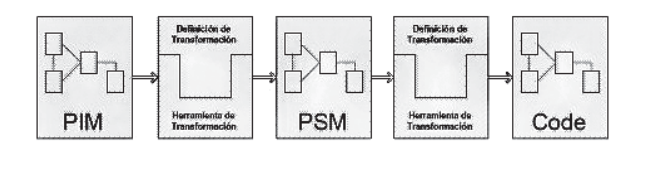
\includegraphics[scale=0.9]{./Imagenes/modelo4}
\caption{Ejemplo de figura 4}
\label{figura4}
\end{figure}

Si abriéramos la herramienta de transformación y mirásemos dentro, podríamos ver qué elementos están involucrados en la ejecución de la transformación. En algún lugar dentro de la herramienta hay una definición que describe como se debe transformar el modelo fuente para producir el modelo destino. Esta es la definición de la transformación. La figura 2-6 muestra la estructura de la herramienta de transformación. Notemos que hay una diferencia entre la transformación misma, que es el proceso de generar un nuevo modelo a partir de otro modelo, y la definición de la transformación. Para especificar la transformación, (que será aplicada muchas veces, independientemente del modelo fuente al que será aplicada) se relacionan construcciones de un lenguaje fuente en construcciones de un lenguaje destino. Se podría, por ejemplo, definir una transformación que relaciona elementos de UML a elementos Java, la cual describiría como los elementos Java pueden ser generados a partir de los elementos UML. Esta situación se muestra en la figura 2-5. DESARROLLO DE SOFTWARE DIRIGIDO POR MODELOS 53 En general, se puede decir que una definición de transformación consiste en una colección de reglas, las cuales son especificaciones no ambiguas de las formas en que un modelo (o parte de él) puede ser usado para crear otro modelo (o parte de él).\\

\begin{figure}[H]
\centering
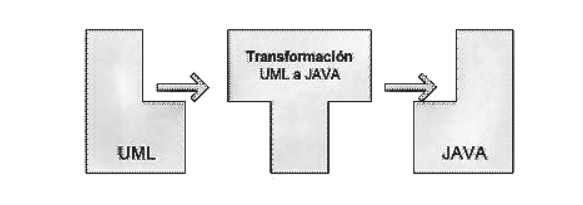
\includegraphics[scale=0.9]{./Imagenes/modelo5}
\caption{Ejemplo de figura 5}
\label{figura5}
\end{figure}

\subsection{¿Cómo se define una transformación?}
 Una transformación entre modelos puede verse como un programa de computadora que toma un modelo como entrada y produce un modelo como salida. Por lo tanto las transformaciones podrían describirse (es decir, implementarse) utilizando cualquier lenguaje de programación, por ejemplo Java. Sin embargo, para simplificar la tarea de codificar transformaciones se han desarrollado lenguajes de más alto nivel (o específicos del dominio de las transformaciones) para tal fin, tales como ATL [ATL] y QVT [QVT].
 
\subsection{Un ejemplo de transformación}
Exhibiremos un ejemplo de una transformación de un modelo PIM escrito en UML a un modelo de implementación escrito en Java. Transformaremos el diagrama de clases de un sistema de venta de libros (Bookstore) en las clases de Java correspondientes a ese modelo. La figura 2-8 muestra gráficamente la transformación que se intenta realizar, la cual consta de 2 pasos: Transformaremos el PIM en un PSM y luego transformaremos el PSM resultante a código Java

\begin{figure}[H]
\centering
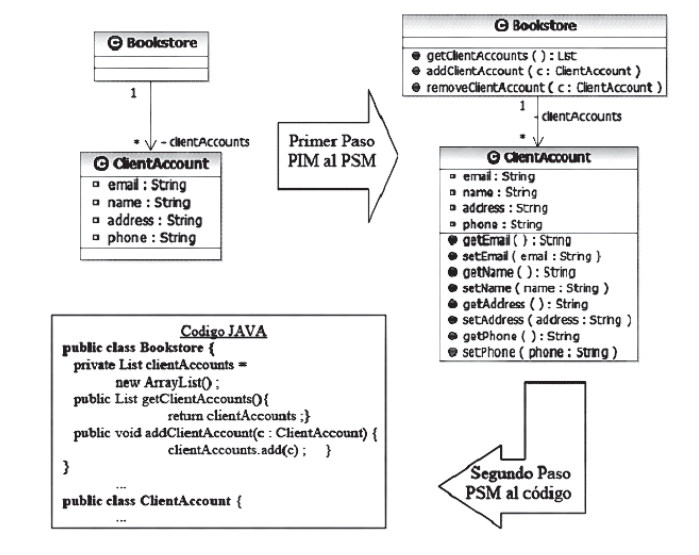
\includegraphics[scale=0.9]{./Imagenes/modelo6}
\caption{Ejemplo de figura 6}
\label{figura6}
\end{figure}

Tanto el PIM como el PSM son modelos útiles ya que proveen el nivel de información adecuado para diferentes tipos de desarrolladores y otras personas involucradas en el proceso de desarrollo de software. Existe una clara relación entre estos modelos. La definición de la transformación que debe aplicarse para obtener el PSM a partir del PIM consiste en un conjunto de reglas. Estas reglas son: \\\\
- Para cada clase en el PIM se genera una clase con el mismo nombre en el PSM. \\
- Para cada relación de composición entre una clase llamada classA y otra clase llamada classB, con multiplicidad 1 a n, se genera un atributo en la clase classA con nombre classB de tipo Collection. \\
- Para cada atributo público definido como attributeName:Type en el PIM los siguientes atributos y operaciones se generan como parte de la clase destino:\\ 
o Un atributo privado con el mismo nombre: attributeName: Type\\ 
o Una operación pública cuyo nombre consta del nombre del atributo\\ precedido con “get” y el tipo del atributo como tipo de retorno: getAttributeName(): Type \\
o Una operación pública cuyo nombre consta del nombre del atributo precedido con “set” y con el atributo como parámetro y sin valor de retorno: setAttributeName(att: Type). \\\\
El siguiente paso consistirá en escribir una transformación que tome como entrada el PSM y lo transforme a código Java. Combinando y automatizando ambas transformaciones podremos generar código Java a partir del PIM

\subsection{Herramientas de soporte para MDD}
 La puesta en práctica del proceso MDD requiere de la disponibilidad de herramientas de software que den soporte a la creación de modelos y transformaciones. La figura 2-9 brinda un panorama de los distintos puntos en los que el proceso MDD necesita ser soportado por herramientas. En particular, necesitamos los siguientes elementos:\\\\ 
- Editores gráficos para crear los modelos ya sea usando UML como otros lenguajes de modelado específicos de dominio.\\
- Repositorios para persistir los modelos y manejar sus modificaciones y versiones. \\
- Herramientas para validar los modelos (consistencia, completitud, etc.).\\
- Editores de transformaciones de modelos que den soporte a los distintos lenguajes de transformación, como QVT o ATL.\\
- Compiladores de transformaciones, debuggers de transformaciones.\\
- Herramientas para verificar y/o testear las transformaciones.

\begin{figure}[H]
\centering
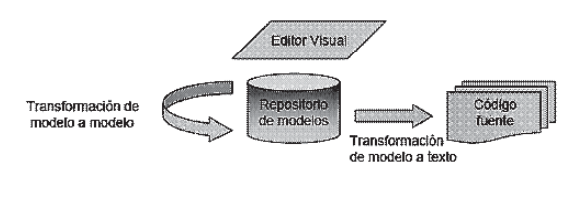
\includegraphics[scale=0.9]{./Imagenes/modelo7}
\caption{Ejemplo de figura 7}
\label{figura7}
\end{figure}



